%% -*- coding: utf-8 -*-
\documentclass[12pt,a4paper]{scrartcl} 
\usepackage[utf8]{inputenc}
\usepackage[english,russian]{babel}
\usepackage{indentfirst}
\usepackage{misccorr}
\usepackage{graphicx}
\usepackage{indentfirst}
\usepackage{amsmath}
\begin{document}
 \begin{titlepage}
  \begin{center}
   \large
   МИНИСТЕРСТВО НАУКИ И ВЫСШЕГО ОБРАЗОВАНИЯ РОССИЙСКОЙ ФЕДЕРАЦИИ
   
   Федеральное государственное бюджетное образовательное учреждение высшего образования
   
   \textbf{АДЫГЕЙСКИЙ ГОСУДАРСТВЕННЫЙ УНИВЕРСИТЕТ}
   \vspace{0.25cm}
   
   Инженерно-физический факультет
   
   Кафедра автоматизированных систем обработки информации и управления
   \vfill

   \vfill
   
   \textsc{Отчет по практике}\\[5mm]
   
   {\LARGE Программаная реализация обратной матрицы. \textit{Вариант 5.}}
   \bigskip
   
   1 курс, группа 1ИВТ2-2
  \end{center}
  \vfill
  
  \newlength{\ML}
  \settowidth{\ML}{«\underline{\hspace{0.7cm}}» \underline{\hspace{2cm}}}
  \hfill\begin{minipage}{0.5\textwidth}
   Выполнила:\\
   \underline{\hspace{\ML}} Е.\,Е.~Бубенщикова\\
   «\underline{\hspace{0.7cm}}» \underline{\hspace{2cm}} 2023 г.
  \end{minipage}%
  \bigskip
  
  \hfill\begin{minipage}{0.5\textwidth}
   Руководитель:\\
   \underline{\hspace{\ML}} С.\,В.~Теплоухов\\
   «\underline{\hspace{0.7cm}}» \underline{\hspace{2cm}} 2023 г.
  \end{minipage}%
  \vfill
  
  \begin{center}
   Майкоп, 2023 г.
  \end{center}
 \end{titlepage}
 
% Содержание
\section{Введение}
\label{sec:intro}


\subsection{Формулировка цели}
Целью данной работы является написание программы для вычисления матрицы обратную заданной.

\subsubsection{Теория}
Нахождение обратной матрицы методом исключения неизвестных Гаусса. Первый шаг для нахождения обратной матрицы методом исключения неизвестных Гаусса - приписать к матрице A единичную матрицу того же порядка, отделив их вертикальной чертой. Мы получим сдвоенную матрицу A|E.  Умножим обе части этой матрицы на A\textasciicircum-1, тогда получим (A*A\textasciicircum-1|E*A\textasciicircum-1), но A*A\textasciicircum-1=E и E*A\textasciicircum-1=A\textasciicircum-1.
Алгоритм нахождения обратной матрицы методом исключения неизвестных Гаусса
    \begin{enumerate}
        \item К матрице A приписать единичную матрицу того же порядка;
        \item Полученную сдвоенную матрицу преобразовать так, чтобы в левой её части получилась единичная матрица, тогда в правой части на месте единичной матрицы автоматически получится обратная матрица. Матрица A в левой части преобразуется в единичную матрицу путём элементарных преобразований матрицы;
        \item Если в процессе преобразования матрицы A в единичную матрицу в какой-либо строке или в каком-либо столбце окажутся только нули, то определитель матрицы равен нулю, и, следовательно, матрица A будет вырожденной, и она не имеет обратной матрицы. В этом случае дальнейшее нахождение обратной матрицы прекращается.
    \end{enumerate}
    \noindent 

\section{Ход работы}
\subsection{Код выполненной программы}

\begin{verbatim}
import numpy as np

# Считываем размерность матрицы
n = int(input("Введите количество строк: "))
m = int(input("Введите количество столбцов: "))

# Считываем элементы матрицы
A = np.zeros((n, m))
for i in range(n):
    for j in range(m):
       A[i, j] = float(input( "Введите элемент [{i + 1}, {j + 1}]"))

# Вычисляем обратную матрицу
det = np.linalg.det(A)
if det == 0:
    print("Матрица необратима")
else:
    A_inv = np.linalg.inv(A)
    if m == n:
        # Если матрица квадратная, выводим обратную матрицу
        print("Обратная матрица: ")
        print(A_inv)
    else:
        # Если матрица прямоугольная, выводим обратную матрицу с округлением до 2 знаков после запятой
        A_inv = np.round(A_inv, 2)
        print("Обратная матрица: ")
        print(A_inv)
\end{verbatim}

\begin{figure}[h]
 \centering
 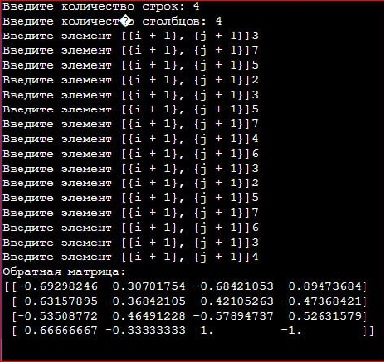
\includegraphics[width=1\textwidth]{photo1686082293.jpeg}
 \caption{Результат работы}\label{fig:par}
\end{figure}






\end{document}